\documentclass{article}

% Bibliography
\usepackage{natbib}
\bibpunct{(}{)}{;}{a}{}{;}

% Use 'It was found that A is B (Name 1234)' style
\setcitestyle{authoryear,open={},close={}}

% Affiliations
\usepackage{authblk}
\title{pirouette: the error BEAST2 makes in inferring a phylogeny}
\author[1]{Rich\`el J.C. Bilderbeek}
\author[1]{Giovanni Laudanno}
\author[1]{Rampal S. Etienne}
\affil[1]{Groningen Institute for Evolutionary Life Sciences, University of Groningen, Groningen, The Netherlands}

% Use double spacing
\usepackage{setspace}
\doublespacing

\usepackage{listings}
\usepackage{hyperref}
\usepackage{todonotes}
\usepackage{verbatim}
\usepackage{pgf}
\usepackage{bm}

% sidewaysfigure
\usepackage{rotating}

% Style of listings
% From http://r.789695.n4.nabble.com/How-to-nicely-display-R-code-with-the-LaTeX-package-listings-tp4648110.html
\usepackage{fancyvrb} 
\definecolor{codegreen}{rgb}{0,0.6,0}
\definecolor{codegray}{rgb}{0.5,0.5,0.5}
\definecolor{codepurple}{rgb}{0.58,0,0.82}
\definecolor{backcolor}{rgb}{0.95,0.95,0.92}
\lstdefinestyle{mystyle}{
  language=R,% set programming language
  basicstyle=\ttfamily\small,% basic font style
  commentstyle=\color{gray},% comment style
  % numbers=left,% display line numbers on the left side
  numberstyle=\scriptsize,% use small line numbers
  numbersep=10pt,% space between line numbers and code
  tabsize=2,% sizes of tabs
  showstringspaces=false,% do not replace spaces in strings by a certain character
  captionpos=b,% positioning of the caption below
  breaklines=true,% automatic line breaking
  escapeinside={(*}{*)},% escaping to LaTeX
  fancyvrb=true,% verbatim code is typset by listings
  extendedchars=false,% prohibit extended chars (chars of codes 128--255)
  alsoletter={.<-},% becomes a letter
  alsoother={$},% becomes other
  otherkeywords={!=, ~, $, \&, \%/\%, \%*\%, \%\%, <-, <<-, /},% other keywords
  deletekeywords={c}% remove keywords 
}
\lstset{style=mystyle}

% Adds numbered lines
\usepackage{lineno}
\linenumbers

% Rename 'Abstract' to 'Summary 
\usepackage[english]{babel}
\addto{\captionsenglish}{\renewcommand{\abstractname}{Summary}}

%comments
\newcommand{\giovanni}[1]{\textcolor{blue}{\textbf{[GL: #1]}}}
\newcommand{\richel}[1]{\textcolor{orange}{\textbf{[RB: #1]}}}

\begin{document}

\maketitle

\begin{abstract}

  \textbf{1. }
    BEAST2 is a popular Bayesian phylogenetics software tool,
    that takes an alignment and inference model to create a
    posterior of jointly-estimated phylogenies and model parameter estimates.
    When a new macro-evolutionary diversification model is developed,
    a good first step is to measure the error BEAST2 makes on a known
    phylogeny derived from a new diversification mechanism, 
    with its current set of inference models. \\
  \textbf{2. }
    Here, we present a free, libre and open-source R package, \verb;pirouette;
    that assesses the inference error BEAST2 makes based on a known/true 
    phylogeny. \\
  \textbf{3. }
    We describe \verb;pirouette;'s usage and the biological scientific
    question it can answer, including full examples. \\
  \textbf{4. }
    As \verb;pirouette; is designed to be of high quality and extendable, 
    we conclude by describing the further development of the package. \\
\end{abstract}

{\bf Keywords:} computational biology, evolution, phylogenetics, BEAST2, pirouette, R





%%%%%%%%%%%%%%%%%%%%%%%%%%%%%%%%%%%%%%%%%%%%%%%%%%%%%%%%%%%%%%%%%%%%%%%%%%%%%%%%%%%%%%
\section{Introduction}
%%%%%%%%%%%%%%%%%%%%%%%%%%%%%%%%%%%%%%%%%%%%%%%%%%%%%%%%%%%%%%%%%%%%%%%%%%%%%%%%%%%%%%

The development of new powerful inference tools, 
such as BEAST [\cite{drummond2007beast}] or MrBayes [\cite{huelsenbeck2001mrbayes}], 
provides us the possibility to build phylogenetic trees 
from genetic material extracted from extant organisms.
This has constituted an important step forward 
in our understanding on how species 
evolve.
Such tools have been increasingly exploited to hypothesize and test what are the main drivers
and modes for diversification processes. 

There are plenty of diversification models: 
constant-birth [Yule, 19..],
birth-death [\cite{nee1994reconstructed}], 
time-dependent [Rabosky D., LASER package?], 
diversity dependent [\cite{etienne2011diversity}], 
protracted birth-death [\cite{rosindell2010protracted}][\cite{etienne2012prolonging}],
multiple-birth death [Laudanno, Bilderbeek, Haegeman \& Etienne, in preparation],
a rate shifting birth-death model [the SLS model. Laudanno, Haegeman \& Etienne, in preparation]
punctuated equilibrium (as known as "early burst") [\cite{harmon2010early}],
dependent on a binary trait [\cite{maddison2007estimating}], 
multiple state trait [\cite{fitzjohn2012diversitree}],
concealed state [\cite{beaulieu2016detecting}] 
or even a combination of multiple concealed and observable states [\cite{herrera2018detecting}].

Such models usually rely on the assumption 
that a particular diversification process 
can be explained mainly by a specific mechanism.
Such a mechanism is built into a likelihood function, 
which provides the likelihood of the parameters, given the data.
By maximizing it, it is possible 
to estimate the what are the best values for model parameters. 
It is a standard practice in assessing such models,
to verify the level of accuracy they can achieve
on simulated phylogenies, of which full knowledge is given.

Diversification models are getting more complex over time. There are many
reasons for this. One reason is the increase in computing power,
which allows this heightened complexity possible.
Another reason is to explore a process that are not yet considered by currently existing diversification models. An example of this
is the multiple-birth model [Laudanno et al., in preparation], 
that is the first model to allow simultaneous speciations to co-occur.

However, whenever a new model is proposed there is always a trade-off between the cost of increased complexity versus the benefits that it can provide.
Therefore desirable models have to be able to disentangle the intrinsic complexity of a system, 
highlight the main reasons of its behaviour and avoid unnecessary complexity. Furthermore developing models can cost time, human and computational resources.

\iffalse
One of the purposes of modelling a complex systems
is to hypothesize the main driving factors of a process 
and trying to prove that they are indeed able 
to explain the main features of the phenomenon you want to explain.
Due to this, there are diminishing returns on adding complexity
to a model: the job of a modeller is to try to
disentangle the intrinsic complexity of a system 
highlighting the main reasons of its behaviour. 
In such a light you don't want your model to be unnecessary complex.
Additionally, developing a likelihood model takes time, 
human resources, fundings and can strain computational resources.
\fi

For this reason we believe it is important to have techniques to quantitatively assess the advancement provided by new models, in comparison to the existing ones.

\iffalse
When assuming that a new diversification model is worth the
(philosophical) effort, there are many ways to measure
if the new model indeed gives a better explanation. 
\fi

To achieve this, one possible experiment
is to simulate a phylogeny according to the mechanisms proposed by the new diversification model, then simulate its alignment and measure how well current inference models perform at retrieving the original phylogeny.
If this difference is small enough, current models apparently
suffice.

\verb;pirouette; is an R package that performs such an experiment,
and is built on \verb;babette; [Bilderbeek \& Etienne, 2018], 
which calls the popular Bayesian inference tool 
BEAST2 [\cite{bouckaert2014beast}]. With \verb;pirouette;, one
can easily measure the error made by Bayesian inference in recovering
any given phylogeny, helping us to validate new diversification models.

%%%%%%%%%%%%%%%%%%%%%%%%%%%%%%%%%%%%%%%%%%%%%%%%%%%%%%%%%%%%%%%%%%%%%%%%%%%%%%%%%%%%%%
\section{Description}
%%%%%%%%%%%%%%%%%%%%%%%%%%%%%%%%%%%%%%%%%%%%%%%%%%%%%%%%%%%%%%%%%%%%%%%%%%%%%%%%%%%%%%

\verb;pirouette; is written in the R programming language (\cite{R}).

\begin{sidewaysfigure}
  \centering
  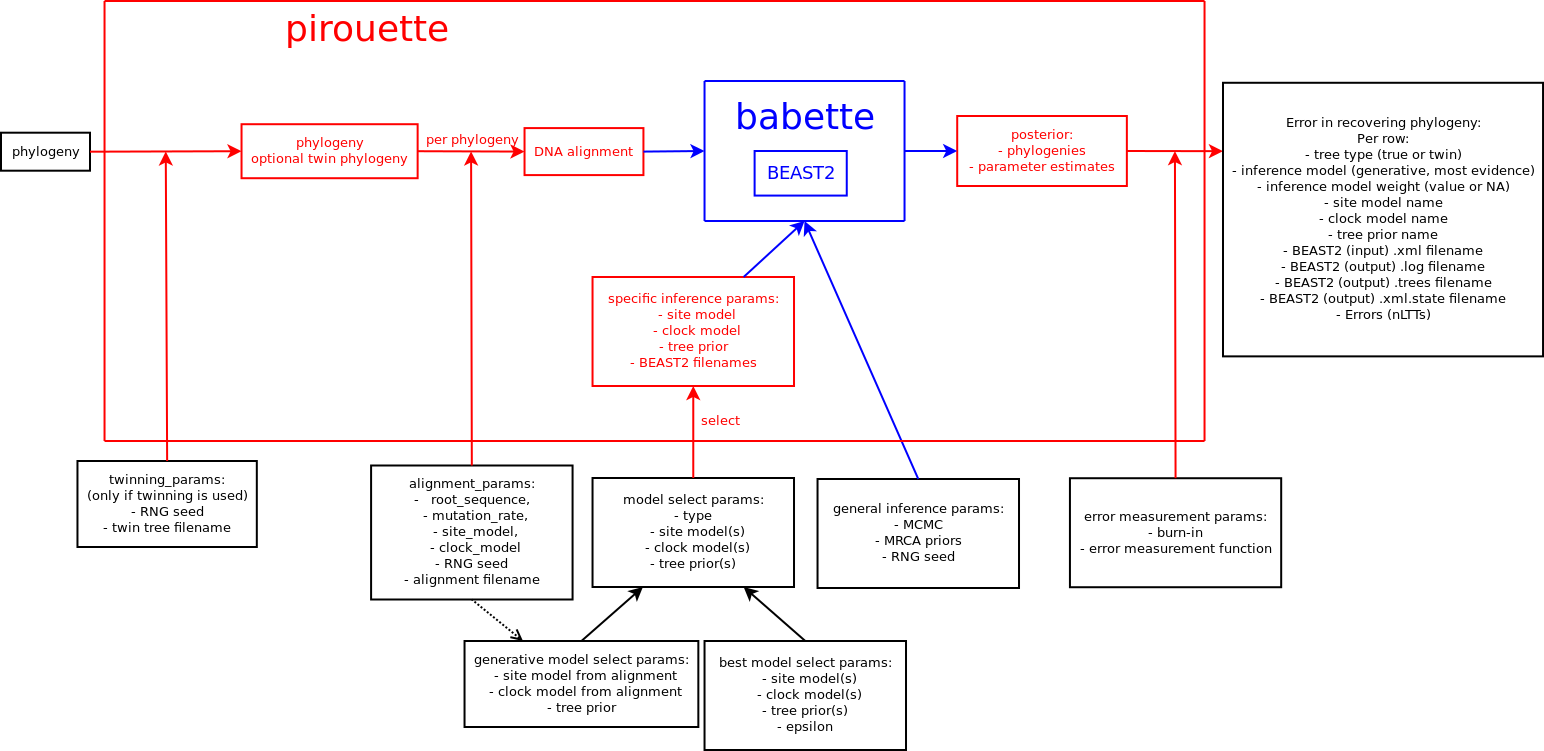
\includegraphics[width=\textwidth]{overview.png}
  \caption{pirouette pipeline}
  \label{fig:pipeline}
\end{sidewaysfigure}

The goal of \verb;pirouette; is to measure the inference error BEAST2
makes from a given reconstructed phylogeny. For this measurement,
two models need to be specified: a generative and an inference model.
A generative model is a combination of site model, clock model and tree prior,
used to simulate alignments. An inference model is a combination of 
site model, clock model, tree prior, an optional node calibration prior
and setup of the Markov chain Monte Carlo (MCMC) algorithm, 
used to produce a posterior. Node calibration priors, called 'most
recent common ancestor' (MRCA) priors within BEAST2 allow to create a 
time-calibrated phylogeny, by specifying a normal distribution around
an expected time when two or more taxa's ancestors diversified. 

The pipeline is summarized by the following steps, which will be described in detail below:
\begin{enumerate}
    \item from a given phylogeny an alignment is simulated;
    \item from the alignment an inference model is chosen;
    \item the alignment is used as BEAST2 input to infer a posterior distribution of phylogenies;
    \item posterior phylogenies are compared with the given original phylogeny to estimate the error we make. The bigger the match, the lower the error;
\end{enumerate}
\richel{figure to pipeline here}
There is also the option to generate a 'twin tree',
that goes through the same pipeline.

The first step simulates a DNA alignment from the given phylogeny.
One can specify a DNA sequence
of any length at the root of the phylogeny, a DNA mutation rate, a
site (i.e. nucleotide substitution) model, 
a clock model, a random number generator (RNG) seed and a location
where the alignment is saved to. This step is relatively fast, but longer
DNA alignments will noticeably slow down the inference step.

The second step selects an inference model, using the alignment.
The user can specify whether to use the generative model or select a best model
from a set of inference models. 
When selecting the generative model,
the site and clock model used in the alignment simulation are used
in the inference. Because the given phylogeny (on which the alignment is based)
may have followed any tree prior (i.e. speciation model), the user needs
to specify which tree prior is used in the inference. 
When selecting for the best
model, the alignment is used to find the inference model that has the
highest evidence (i.e. marginal likelihood) from a set of candidate inference models.
The evidence of an inference model is estimated using a nested sampling (NS)
approach, as described in \cite{maturana2018model}. The nested sampling is
performed by \verb;mcbette; \cite{mcbette}, that calls the 'NS' BEAST2 package. 
Using BEAST2 packages (in a scripted way) can only be done under Linux and Mac; 
inference model selection is not available on Windows.

The third step infers a Bayesian posterior from the simulated alignment,
using the inference model(s) selected in the previous step. The user
can specify the additional parameters needed for the BEAST2 run, which
are the Markov-Chain Monte Carlo (MCMC) setup, 
an optional Most Recent Common Ancestor (MRCA) prior and an RNG seed.
The MCMC setup determines the number of posterior trees sampled.
An MRCA prior allows the inferred phylogeny to have a dated crown age.

The fourth step measures the inference error, using the phylogenies in the
Bayesian posterior. These phylogenies are compared to the given
original phylogeny using an error statistic, which is the nLTT 
statistic (\cite{janzen2015approximate}) by default,
but also a custom error statistic is supplied, based
on the absolute difference in the gamma statistic [Pybus \& Harvy]. 
Additionally, the user can specify the
proportion of posterior phylogenies to 
discard (i.e. the burn-in), throwing away the first $10\%$
of all phylogenies by default. This burn-in is used to discard
the part of the MCMC chain that has not yet converged to a
representative part of state space.

An optional step is to generate a 'twin tree', that will be
analyzed in the same way as the true tree. The twin tree has the same
topology as the given phylogeny, yet its branch lengths follow the same
distribution as a Yule (pure-birth) or (constant rate) birth-death tree prior.
The use of such a twin tree, is to assess the minimum level of noise (i.e. 
error) BEAST2 makes when the input (the twin phylogeny) has an ideal branch
length distribution.

%%%%%%%%%%%%%%%%%%%%%%%%%%%%%%%%%%%%%%%%%%%%%%%%%%%%%%%%%%%%%%%%%%%%%%%%%%%%%%%%%%%%%%
\section{Installation}
%%%%%%%%%%%%%%%%%%%%%%%%%%%%%%%%%%%%%%%%%%%%%%%%%%%%%%%%%%%%%%%%%%%%%%%%%%%%%%%%%%%%%%

\verb;pirouette; can be installed easily from CRAN:

\begin{lstlisting}[language=R, floatplacement=H, frame=single]
install.packages("pirouette")
\end{lstlisting}

For the most up-to-date version, 
one can download and install the package from \verb;pirouette;'s GitHub repository:

\begin{lstlisting}[language=R, floatplacement=H, frame=single]
usethis::install_github("richelbilderbeek/pirouette")
\end{lstlisting}

To start using \verb;pirouette;, load its functions in the global namespace first:

\begin{lstlisting}[language=R, floatplacement=H, frame=single]
library(pirouette)
\end{lstlisting}
Because \verb;pirouette; calls BEAST2, BEAST2 must be installed. 
This can be done from within R, using:

\begin{lstlisting}[language=R, floatplacement=H, frame=single]
install_beast2()
\end{lstlisting}
For the option to select inference models,
\verb;pirouette; uses the "NS" BEAST2 package [\cite{maturana2018model}].
It can be installed from within R, using:

\begin{lstlisting}[language=R, floatplacement=H, frame=single]
install_beast2_pkg("NS")
\end{lstlisting}

%%%%%%%%%%%%%%%%%%%%%%%%%%%%%%%%%%%%%%%%%%%%%%%%%%%%%%%%%%%%%%%%%%%%%%%%%%%%%%%%%%%%%%
\section{Usage: first research question}
%%%%%%%%%%%%%%%%%%%%%%%%%%%%%%%%%%%%%%%%%%%%%%%%%%%%%%%%%%%%%%%%%%%%%%%%%%%%%%%%%%%%%%

A first research question that \verb;pirouette; answers is:
What is the error BEAST2 makes from a phylogeny using the same 
diversification model as it was generated by?

We start with an idealised 
birth-death tree of five taxa and a crown age of 10.
By idealized, we mean a phylogeny that is easiest to recover
by the Bayesian inference. A phylogeny that is easy to recover has
the most common branch length distribution imaginable. We
use an idealised tree, as we want to measure the baseline noise; that is,
the lowest error that BEAST2 can possibly make.

\begin{lstlisting}[language=R, floatplacement=H, frame=single]
phylogeny <- ape::read.tree(text = "((A:7.1,(B:2.2,C:2.2):4.9):2.9,(D:4.6,E:4.6):5.4):0;")
\end{lstlisting}

\begin{figure}[h]
  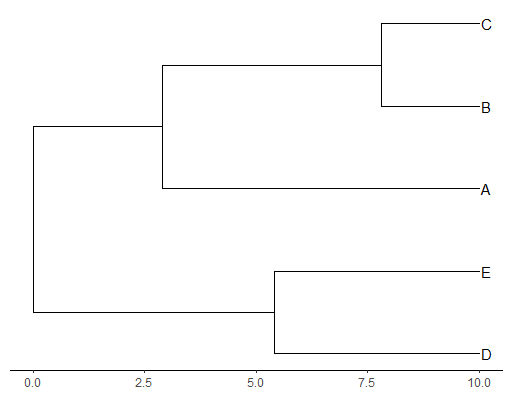
\includegraphics[width=\textwidth]{figure_bd.png}
  \caption{pippo}
\end{figure}

The first step in \verb;pirouette; is to simulate a DNA alignment from the 
given phylogeny. To do so, we must specify the DNA root sequence
and a mutation rate. In this example, the DNA root sequence consists
out of four block of 250 nucleotides each, where the per-nucleotide
mutation rate is 0.1 mutations per unit time.

\begin{lstlisting}[language=R, floatplacement=H, frame=single]
alignment_params <- create_alignment_params(
  root_sequence = create_blocked_dna(length = 1000),
  mutation_rate = 0.1
)
\end{lstlisting}

By default, an alignment is created using a Jukes-Cantor (JC) site model
and a strict clock model. A JC site model assumes that mutations
between all nucloetides are constant at an equal rate. 
A strict clock model assumes that
the mutation rate of all species is equal and constant.
Due to this, we state that the generative model for the alignment is
a JC site model and a strict clock model.

In the second step we state our experiments. In this context, we
define an experiment as a combination of an inference model
and the conditions under which a Bayesian inference is created.

\begin{table}
  \begin{tabular}{ | c | c | c | l | }
    \hline
    \textbf{model type} & \textbf{run if} & \textbf{measure evidence} & \textbf{inference model} \\ 
    \hline
    generative & always & no & generative model \\
    \hline
  \end{tabular}
  \caption{Experimental setup to answer the first research question}
\end{table}

If we know how the generative model of the alignment, as we did above,
we can re-use that information. We do still need to specify 
a generative tree prior, which is the tree prior underlying the phylogeny.
In this case, we'll pick a (constant-rate) birth-death model:

\begin{lstlisting}[language=R, floatplacement=H, frame=single]
model_select_param <- create_gen_model_select_param(
  alignment_params = alignment_params,
  tree_prior = create_bd_tree_prior()
)
\end{lstlisting}

The third and fourth step have sensible defaults, and we are not
interested in using a twin tree. We can now measure the errors BEAST2
makes when inferring the given phylogeny in this way:

\begin{lstlisting}[language=R, floatplacement=H, frame=single]
errors <- pir_run(
  phylogeny,
  alignment_params = alignment_params,
  model_select_params = model_select_param
)
\end{lstlisting}

\verb;pirouette; has a nice plotting function:

\begin{lstlisting}[language=R, floatplacement=H, frame=single]
pir_plot(errors)
\end{lstlisting}

The resulting figure is shown in figure 2.

\richel{Update figure 2 to use idealized tree}
\giovanni{
  Check "pirouettepackage" repo. 
  I uploaded a function to create the idealized tree that you might like.
}

\begin{figure}[h]
  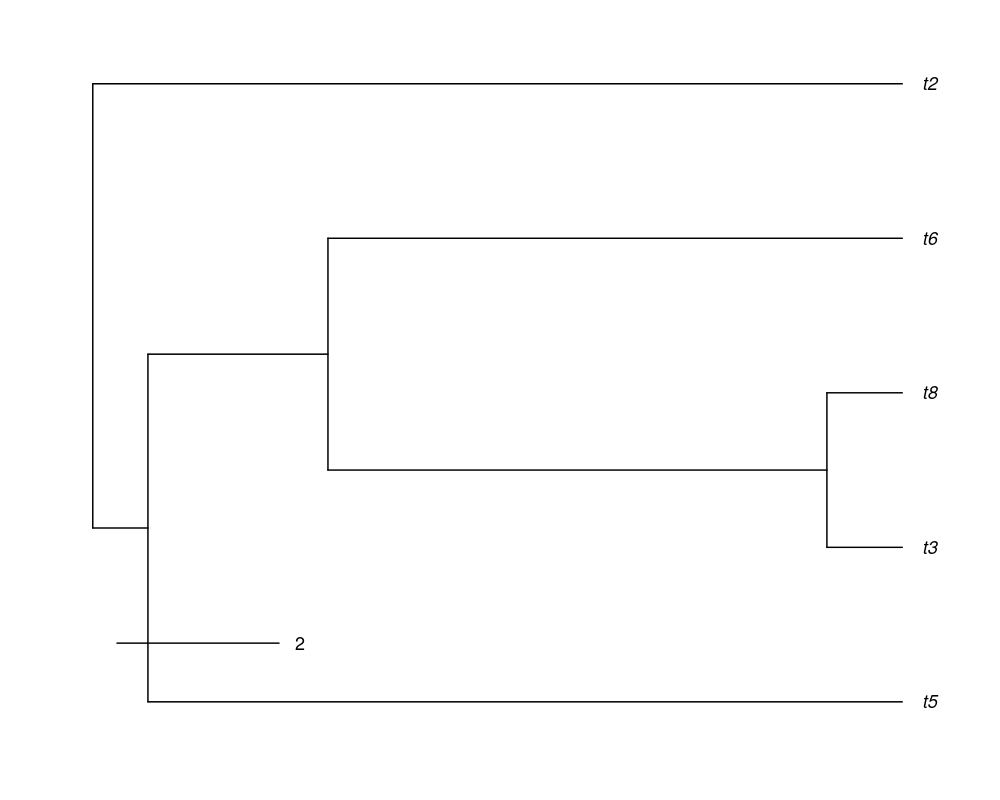
\includegraphics[width=\textwidth]{figure_2.png}
  \caption{
    The error BEAST2 makes from a phylogeny 
    when the generative and inference model are the same
  }
\end{figure}

%%%%%%%%%%%%%%%%%%%%%%%%%%%%%%%%%%%%%%%%%%%%%%%%%%%%%%%%%%%%%%%%%%%%%%%%%%%%%%%%%%%%%%
\section{Usage: second research question}
%%%%%%%%%%%%%%%%%%%%%%%%%%%%%%%%%%%%%%%%%%%%%%%%%%%%%%%%%%%%%%%%%%%%%%%%%%%%%%%%%%%%%%

A second research question that \verb;pirouette; answers, is:
What is the error BEAST2 makes from a phylogeny when
picking the best inference model?

Here we start with a tree generated from an unknown 
diversification model, that has four taxa and a crown age of 5:

% Need idealised birth-death tree
% From https://github.com/richelbilderbeek/pirouette_article/issues/1
% and https://github.com/richelbilderbeek/pirouette/issues/35
\begin{lstlisting}[language=R, floatplacement=H, frame=single]
phylogeny <- ape::read.tree(text = "((A:4, B:4):1, (C:4, D:4):1);")
\end{lstlisting}

The first step in \verb;pirouette; is to simulate a DNA alignment from the 
given phylogeny. We'll re-use the alignment parameters of the previous example 
\richel{TODO: add ref to code}
 
The second step is to select how an inference model is picked.
We will let the inference model that has the highest evidence to be used
in the Bayesian inference. By default, \verb;pirouette; will use
its full arsenal of 40 inference models, which are all combinations of 4 site 
models, 2 clock models and 5 tree priors.

\begin{lstlisting}[language=R, floatplacement=H, frame=single]
model_select_param <- create_best_model_select_param()
\end{lstlisting}

Also here, the third and fourth step have sensible defaults, and we are not
interested in using a twin tree. We can now measure the errors BEAST2
makes when inferring the given phylogeny like this:

\begin{lstlisting}[language=R, floatplacement=H, frame=single]
errors <- pir_run(
  phylogeny,
  alignment_params = alignment_params,
  model_select_params = model_select_param
)
\end{lstlisting}

Again, showing the results:

\begin{lstlisting}[language=R, floatplacement=H, frame=single]
pir_plot(errors)
\end{lstlisting}

The resulting figure is shown in figure 3.

\begin{figure}[h]
  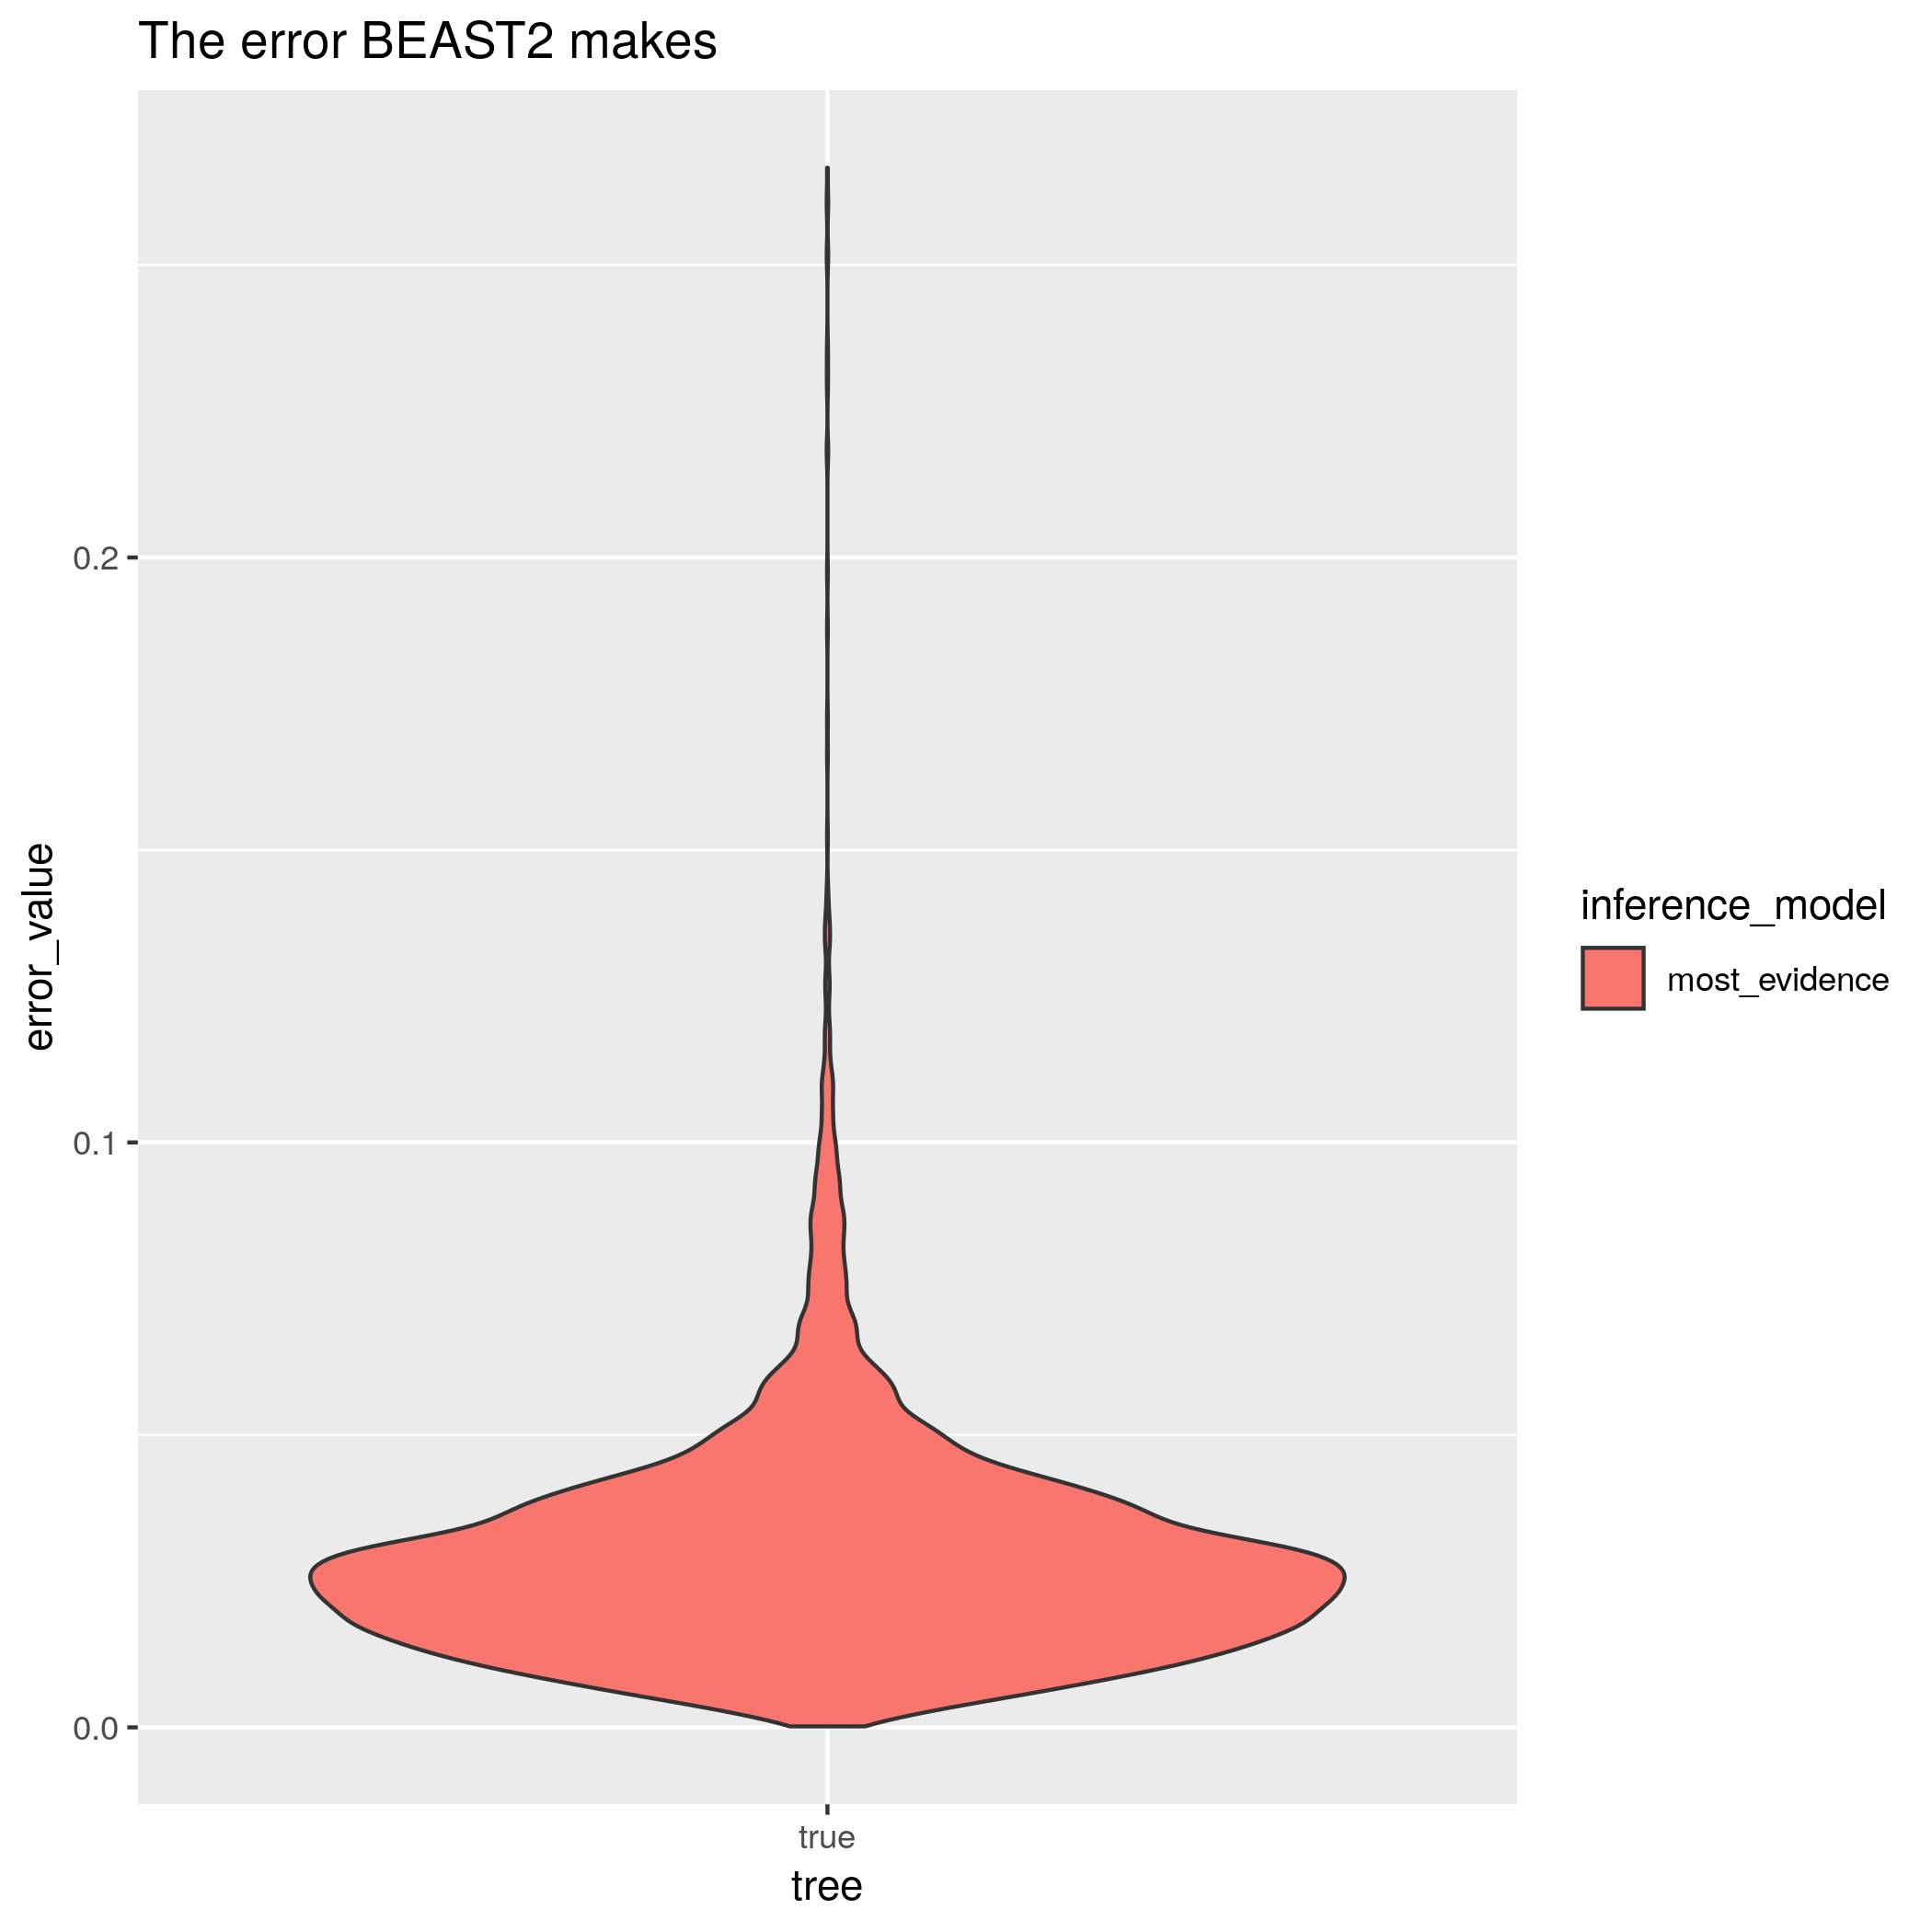
\includegraphics[width=\textwidth]{figure_3.png}
  \caption{
    The error BEAST2 makes from a phylogeny when
    picking the best inference model
  }
\end{figure}

%%%%%%%%%%%%%%%%%%%%%%%%%%%%%%%%%%%%%%%%%%%%%%%%%%%%%%%%%%%%%%%%%%%%%%%%%%%%%%%%%%%%%%
\section{Usage: third research question}
%%%%%%%%%%%%%%%%%%%%%%%%%%%%%%%%%%%%%%%%%%%%%%%%%%%%%%%%%%%%%%%%%%%%%%%%%%%%%%%%%%%%%%

A third research question that \verb;pirouette; answers is:
What is the error BEAST2 makes from a phylogeny 
picking the best inference model, compared to the background noise?

The following settings are the same as in the previous section:
phylogeny, alignment parameters, inference model selection,
shared inference parameters and error measuring parameters 
\richel{TODO: add ref to code}

This time, we are interested in creating a twin tree. A twin tree
has the same topology as the given tree, yet its branch lengths follow
an idealized 
\giovanni{
  I don't think this is true. A twin tree is generated randomly. 
  If we use the method "maxlikelihood" (see the function "createbdtree") 
  the tree will be chosen in such a way it will maximizing the likelihood 
  given the parameters we estimated from the original tree, 
  but I would not call it "idealized". Furthermore I think it's not obvious to 
  use the "maxlikelihood" method, as in general the "ideal" scenario should be 
  established using a distribution of trees. A single tree is always the result 
  of a stochastic process.
}
\richel{we'll discuss this today} 
birth-death distribution. Creating a twinning parameter is easy,
as it has sensible default settings:

\begin{lstlisting}[language=R, floatplacement=H, frame=single]
twinning_params <- create_twinning_params()
\end{lstlisting}

We can now measure the errors BEAST2
makes when inferring the given phylogeny, compared
to the background noise, like this:

\begin{lstlisting}[language=R, floatplacement=H, frame=single]
errors <- pir_run(
  phylogeny,
  twinning_params = twinning_params,
  alignment_params = alignment_params,
  model_select_params = model_select_param
)
\end{lstlisting}

Again, showing the results:

\begin{lstlisting}[language=R, floatplacement=H, frame=single]
pir_plot(errors)
\end{lstlisting}

The resulting figure is shown in figure 4

\begin{figure}[h]
  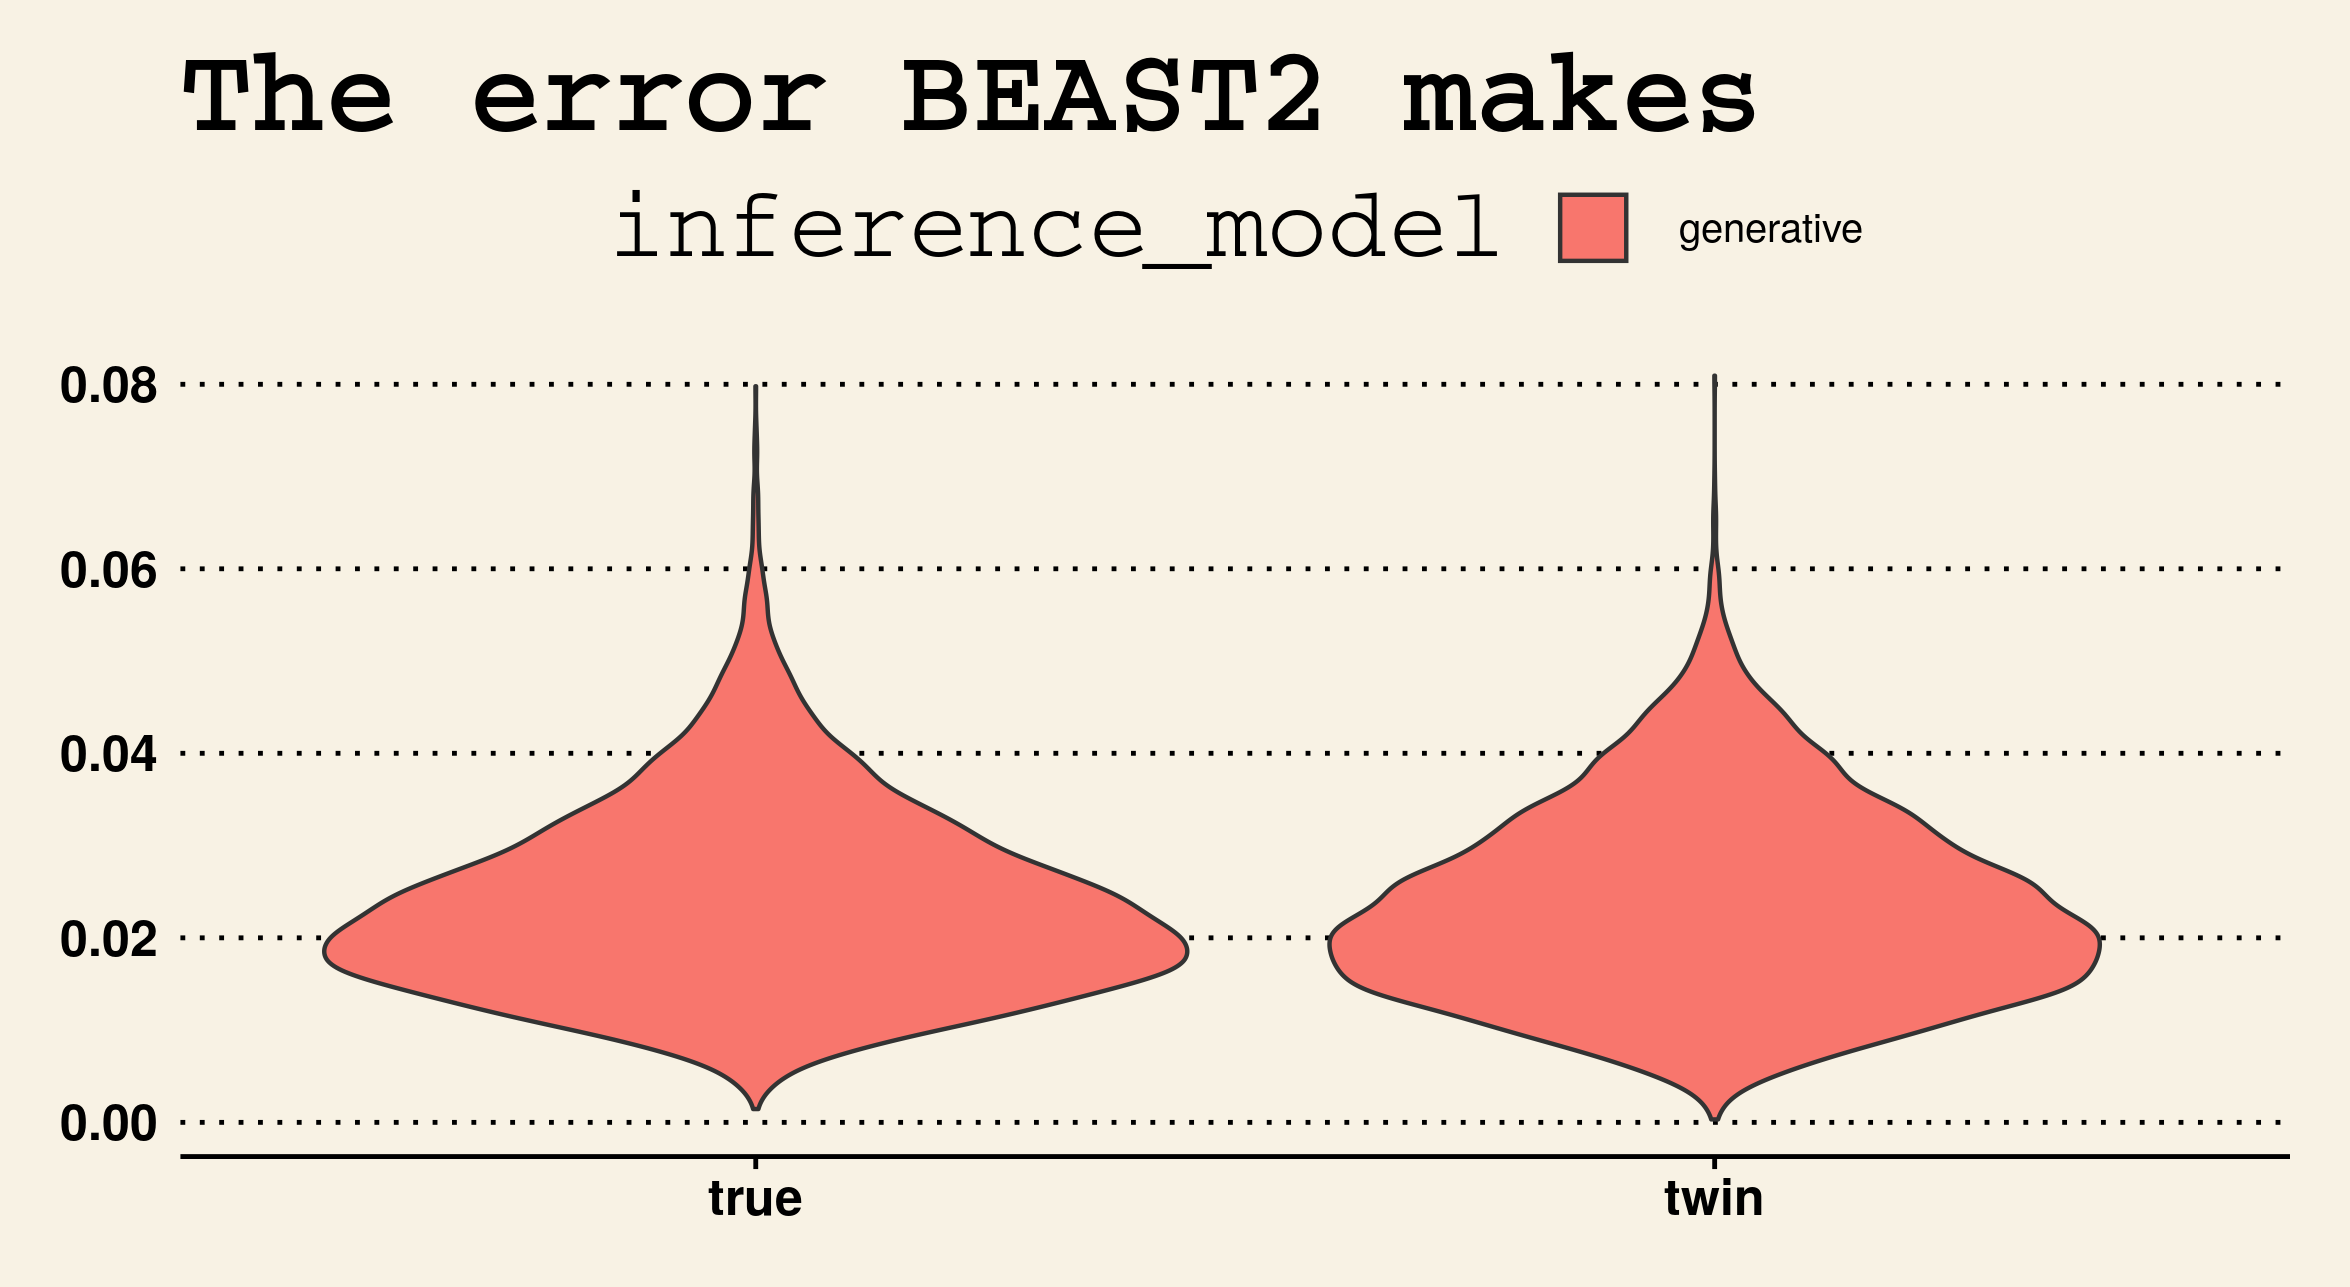
\includegraphics[width=\textwidth]{figure_4.png}
  \caption{
    The error BEAST2 makes from a phylogeny 
    picking the best inference model, compared to the background noise?
    Here, the twin column shows the error BEAST2 makes on an idealized
    tree, to measure the noise, which is the minimal error. 
    \giovanni{again, I don't believe that using an "idealized" tree is the best 
      thing to do. I would rather use more "true trees".}
    \richel{we'll discuss this today}
  }
\end{figure}

%%%%%%%%%%%%%%%%%%%%%%%%%%%%%%%%%%%%%%%%%%%%%%%%%%%%%%%%%%%%%%%%%%%%%%%%%%%%%%%%%%%%%%
\section{Discussion}
%%%%%%%%%%%%%%%%%%%%%%%%%%%%%%%%%%%%%%%%%%%%%%%%%%%%%%%%%%%%%%%%%%%%%%%%%%%%%%%%%%%%%%

\giovanni{We need to discuss the results we got from the 3 experiments.}
\richel{Only iff the journal requires this}

%%%%%%%%%%%%%%%%%%%%%%%%%%%%%%%%%%%%%%%%%%%%%%%%%%%%%%%%%%%%%%%%%%%%%%%%%%%%%%%%%%%%%%
\section{pirouette resources}
%%%%%%%%%%%%%%%%%%%%%%%%%%%%%%%%%%%%%%%%%%%%%%%%%%%%%%%%%%%%%%%%%%%%%%%%%%%%%%%%%%%%%%

\verb;pirouette; is free, libre and open source software available at 
\url{http://github.com/richelbilderbeek/pirouette}
and is licensed under the GNU General Public License v3.0.
\verb;pirouette; uses the Travis CI (\url{https://travis-ci.org})
continuous integration service, which is known to significantly 
increase the number of bugs exposed (\cite{vasilescu2015}) and increases
the speed at which new features are added (\cite{vasilescu2015}).
\verb;pirouette; has a 100\% code coverage, which correlates with 
code quality (\cite{horgan1994,del1995correlation}). 
\verb;pirouette; follows Hadley Wickham's style guide (\cite{style_guide}), 
which improves software quality (\cite{fang2001}).
\verb;pirouette; depends on multiple packages, which are 
\verb;ape; (\cite{APE}), 
\verb;babette; (\cite{bilderbeek2018babette}),
\verb;ggplot2; (\cite{ggplot2}),
\verb;knitr; (\cite{knitr}),
\verb;mcbette; (\cite{mcbette}),
\verb;phangorn; (\cite{phangorn}),
\verb;rmarkdown; (\cite{rmarkdown}),
\verb;stringr; (\cite{stringr}),
\verb;testit; (\cite{testit}) and 
\verb;usethis; (\cite{usethis}).

\verb;pirouette;'s development takes place on GitHub,
\url{https://github.com/richelbilderbeek/pirouette}, 
which accommodates collaboration (\cite{perez2016ten}) 
and improves transparency (\cite{gorgolewski2016practical}).
\verb;pirouette;'s GitHub facilitates feature requests and 
has guidelines on how to do so.

\verb;pirouette;'s documentation is extensive. All functions are documented
in the package's internal documentation. For quick use, 
each exported function shows a minimal example. 
For easy exploration, each exported function's documentation links to related functions.
Additionally, \verb;pirouette; has a vignette that demonstrates extensively how
to use it. 

%%%%%%%%%%%%%%%%%%%%%%%%%%%%%%%%%%%%%%%%%%%%%%%%%%%%%%%%%%%%%%%%%%%%%%%%%%%%%%%%%%%%%%
\section{Citation of pirouette}
%%%%%%%%%%%%%%%%%%%%%%%%%%%%%%%%%%%%%%%%%%%%%%%%%%%%%%%%%%%%%%%%%%%%%%%%%%%%%%%%%%%%%%

Scientists using \verb;pirouette; in a published paper can cite this
article, and/or cite the \verb;pirouette; package 
directly. To obtain this citation from within an R script, use:

\begin{lstlisting}[language=R]
> citation("pirouette")
\end{lstlisting}

%%%%%%%%%%%%%%%%%%%%%%%%%%%%%%%%%%%%%%%%%%%%%%%%%%%%%%%%%%%%%%%%%%%%%%%%%%%%%%%%%%%%%%
\section{Acknowledgements}
%%%%%%%%%%%%%%%%%%%%%%%%%%%%%%%%%%%%%%%%%%%%%%%%%%%%%%%%%%%%%%%%%%%%%%%%%%%%%%%%%%%%%%

We would like to thank the Center for Information Technology of the University 
of Groningen for their support and for providing access to the Peregrine 
high performance computing cluster. 
We thank the Netherlands 
Organization for Scientific Research (NWO) for financial support 
through a VICI grant awarded to RSE.

%%%%%%%%%%%%%%%%%%%%%%%%%%%%%%%%%%%%%%%%%%%%%%%%%%%%%%%%%%%%%%%%%%%%%%%%%%%%%%%%%%%%%%
\section{Data Accessibility}
%%%%%%%%%%%%%%%%%%%%%%%%%%%%%%%%%%%%%%%%%%%%%%%%%%%%%%%%%%%%%%%%%%%%%%%%%%%%%%%%%%%%%%

All code is archived at \url{http://github.com/richelbilderbeek/pirouette_article},
with DOI \url{https://doi.org/12.3456/zenodo.1234567}.

%%%%%%%%%%%%%%%%%%%%%%%%%%%%%%%%%%%%%%%%%%%%%%%%%%%%%%%%%%%%%%%%%%%%%%%%%%%%%%%%%%%%%%
\section{Authors' contributions}
%%%%%%%%%%%%%%%%%%%%%%%%%%%%%%%%%%%%%%%%%%%%%%%%%%%%%%%%%%%%%%%%%%%%%%%%%%%%%%%%%%%%%%

RJCB, GL and RSE conceived the idea for the package. 
RJCB created and tested the package, and wrote the first draft of the manuscript.
GL tested the package and contributed substantially to revisions.
RSE contributed to revisions.

%%%%%%%%%%%%%%%%%%%%%%%%%%%%%%%%%%%%%%%%%%%%%%%%%%%%%%%%%%%%%%%%%%%%%%%%%%%%%%%%%%%%%%
% Bibliography
%%%%%%%%%%%%%%%%%%%%%%%%%%%%%%%%%%%%%%%%%%%%%%%%%%%%%%%%%%%%%%%%%%%%%%%%%%%%%%%%%%%%%%
% MEE style
\bibliographystyle{mee}
\bibliography{article}
%%%%%%%%%%%%%%%%%%%%%%%%%%%%%%%%%%%%%%%%%%%%%%%%%%%%%%%%%%%%%%%%%%%%%%%%%%%%%%%%%%%%%%

\end{document}
